\documentclass[theme=teal]{khmermath}
\usepackage{needspace}

\geometry{left=0.85cm, right=0.85cm, top=0.60cm, bottom=1.30cm, footskip=0.70cm}
\usepackage{colortbl}
\usepackage{tikz}
\usetikzlibrary{calc,shapes,arrows,intersections,through,backgrounds,shadows,decorations.pathmorphing,angles,quotes}

% -------------------------------------------------------------------------
% Korean Math Textbook Style Color Palette & Macros
% -------------------------------------------------------------------------
\definecolor{koreaTeal}{RGB}{0, 150, 155}       % Primary Header Teal/Cyan
\definecolor{koreaDarkTeal}{RGB}{0, 105, 110}   % Dark Teal Accent
\definecolor{koreaBeige}{RGB}{247, 244, 237}     % Concept Sidebar Beige (#F7F4EE)
\definecolor{koreaBeigeBorder}{RGB}{225, 218, 205}
\definecolor{koreaOrange}{RGB}{235, 115, 30}     % Problem Number Orange
\definecolor{koreaBlue}{RGB}{35, 110, 190}      % Standard Blue
\definecolor{koreaPurple}{RGB}{125, 50, 160}    % Purple Accent
\definecolor{koreaNumber}{RGB}{115, 125, 135}   % Problem Number Gray
\definecolor{koreaYellow}{RGB}{255, 246, 175}   % Yellow Highlight Tint

\definecolor{brandNavy}{RGB}{0, 105, 110}
\definecolor{brandBlue}{RGB}{0, 150, 155}
\definecolor{brandLightBlue}{RGB}{247, 244, 237}
\definecolor{brandCrimson}{RGB}{195, 35, 60}
\definecolor{brandCoral}{RGB}{235, 80, 75}
\definecolor{brandGold}{RGB}{215, 130, 10}
\definecolor{brandGoldBg}{RGB}{255, 252, 242}
\definecolor{brandTeal}{RGB}{0, 150, 155}
\definecolor{brandTealBg}{RGB}{244, 252, 250}
\definecolor{subtleGray}{RGB}{248, 249, 250}
\definecolor{cardBorder}{RGB}{220, 212, 198}

% Custom Header & Footer setup (Korean Textbook Style)
\usepackage{fancyhdr}
\pagestyle{fancy}
\fancyhf{}
\renewcommand{\headrulewidth}{0pt}
\renewcommand{\footrule}{\color{koreaTeal!60}\hrule height 0.6pt\vspace{2.5pt}}

\fancyfoot[L]{%
  \fontsize{8}{8}\selectfont\kml \color{koreaNumber}\textbf{\thepage}\ \vline\ \color{koreaDarkTeal}\textbf{មេរៀនទី ៥ ៖ វិសមីការដឺក្រេទី១ មានមួយអញ្ញាត}%
}
\fancyfoot[C]{%
  \fontsize{8}{8}\selectfont\kby \color{koreaDarkTeal}\textbf{\ding{72}\ រៀបរៀងដោយ ៖ \textcolor{koreaDarkTeal}{សុក ពេញ}\ \ding{72}}%
}
\fancyfoot[R]{%
  \fontsize{8}{8}\selectfont\kby \color{koreaDarkTeal}\textbf{ក្លឹបសិក្សាគណិតវិទ្យា \textcolor{brandCrimson}{PCM}}\ \vline\ \color{koreaNumber}\textbf{\thepage}%
}

% Korean Header Banner
\newcommand{\koreanheader}[2]{%
  \noindent%
  \begin{tikzpicture}[x=1cm, y=1cm]
    \fill[koreaTeal, rounded corners=12pt] (0, 0.1) -- (0, 0.95) -- (3.8, 0.95) [rounded corners=0pt] -- (4.4, 0.1) -- cycle;
    \node[white, font=\fontsize{11}{11}\selectfont\kml\bfseries] at (1.9, 0.52) {#1};
    \node[anchor=west, font=\fontsize{16}{16}\selectfont\kml\bfseries, color=koreaDarkTeal] at (4.6, 0.42) {#2};
    \node[anchor=east, font=\fontsize{8.5}{8.5}\selectfont\kby, color=gray!80] at (19.2, 0.48) {$>$ ក្លឹបសិក្សាគណិតវិទ្យា ភី ស៊ី​ អឹម};
  \end{tikzpicture}%
  \vspace{1pt}%
}

% Yellow Formula Highlight Box
\newcommand{\koreahl}[1]{\colorbox{koreaYellow}{\fontsize{8.5}{8.5}\selectfont #1}}

% General Rule Box (Teal/Emerald Theme - ជាទូទៅ)
\newtcolorbox{khboxorange}[1][]{
  enhanced,
  colframe=brandNavy!40,
  colback=brandLightBlue,
  boxrule=0.7pt,
  arc=4.5pt,
  borderline west={3.5pt}{0pt}{brandNavy},
  drop fuzzy shadow=brandNavy!15,
  left=7pt, right=7pt, top=3pt, bottom=2.5pt,
  title={\fontsize{9}{9}\selectfont\kml\color{white}\ding{72}\ ជាទូទៅ},
  coltitle=white,
  colbacktitle=brandNavy,
  boxed title style={
    boxrule=0pt,
    arc=3pt,
    left=6pt, right=6pt, top=2pt, bottom=2pt
  },
  attach boxed title to top left={yshift*=-\tcboxedtitleheight/2, xshift=12pt},
  #1
}

% Practice Card Box
\newtcolorbox{khboxpractice}[1][]{
  enhanced,
  colframe=brandTeal,
  colback=brandTealBg,
  boxrule=0.8pt,
  arc=4pt,
  left=7pt, right=7pt, top=3pt, bottom=3pt,
  #1
}

% Example / Card Item Box
\newtcolorbox{khcard}[1][]{
  enhanced,
  colframe=cardBorder,
  colback=white,
  boxrule=0.7pt,
  arc=3.5pt,
  left=6pt, right=6pt, top=3pt, bottom=3pt,
  #1
}

% Section Badge Macro
\newcommand{\khsection}[2]{%
  \Needspace*{2.5cm}%
  \vspace{1.5pt}%
  \noindent%
  \begin{tikzpicture}
    \fill[rounded corners=4.5pt, brandNavy!8] (0,0) rectangle (19.3, 0.56);
    \fill[rounded corners=3.5pt, brandNavy] (0.05, 0.05) rectangle (0.48, 0.48);
    \node[white, font=\fontsize{9}{9}\selectfont\bfseries] at (0.26, 0.26) {#1};
    \fill[brandGold, rounded corners=1pt] (0.58, 0.10) rectangle (0.62, 0.44);
    \node[anchor=west, font=\fontsize{10}{10}\selectfont\kml, color=brandCrimson] at (0.70, 0.26) {\textbf{#2}};
  \end{tikzpicture}%
  \vspace{1pt}%
}

\def\splitnum#1#2{%
  \color{koreaNumber!65}#1\color{koreaOrange}#2%
}
\newcommand{\koreannum}[1]{%
  \ifstrempty{#1}{}{%
    \mbox{%
      \fontsize{13}{13}\selectfont\bfseries%
      \ifnum#1<10\relax%
        \color{koreaNumber!65}0\color{koreaOrange}#1%
      \else%
        \expandafter\splitnum#1%
      \fi%
    }\,\ %
  }%
}

% Sub-question Badge (Crimson Rounded Square)
\newcommand{\khlabel}[1]{%
  \tikz[baseline=-0.55ex]{%
    \node[fill=brandCrimson, rounded corners=2.5pt, inner sep=1.5pt, minimum width=1.15em, minimum height=1.1em, text=white, font=\kml\fontsize{7}{7}\selectfont, align=center] (lbl) {\raisebox{0.2pt}{#1}};%
  }\,\ %
}

\newcommand{\khbadge}[2]{%
  \tikz[baseline=-0.6ex]{%
    \node[fill=#1, rounded corners=3pt, inner sep=2pt, text=white, font=\kml\fontsize{7}{7}\selectfont] {#2};%
  }%
}
\newcommand{\badgebasic}{\khbadge{brandNavy}{កម្រិតគ្រឹះ}}
\newcommand{\badgestandard}{\khbadge{brandBlue}{កម្រិតមធ្យម}}
\newcommand{\badgeadvanced}{\khbadge{koreaPurple}{កម្រិតខ្ពស់}}
\newcommand{\exhead}[1]{\hangindent=18pt\hangafter=1\koreannum{#1}}

% Comparison Box Marker (Square for filling)
\newcommand{\khboxfill}{\tikz[baseline=-0.6ex]\draw[thick, color=brandNavy, fill=white, rounded corners=2pt] (0,0) rectangle (0.55, 0.44);}

\setlength{\parindent}{0pt}
\setlength{\parskip}{0.8pt}
\setlength{\columnsep}{14pt}
\setlength{\columnseprule}{0.5pt}
\def\columnseprulecolor{\color{koreaTeal!35}}

\begin{document}

% =========================================================================
% PAGE 1: ផ្នែកទី ១ ៖ លក្ខណៈនៃវិសមភាព (Two-column Korean Style)
% =========================================================================
\koreanheader{មេរៀនទី ៥}{វិសមីការដឺក្រេទី១ មានមួយអញ្ញាត}

\khsection{១}{លក្ខណៈនៃវិសមភាព (Properties of Inequality)}

\begin{khboxorange}
  \begin{minipage}[c]{0.68\textwidth}
    \begin{itemize}[leftmargin=12pt, itemsep=1pt, topsep=1pt, parsep=0pt]
      \item[\color{brandNavy}\ding{228}] \textbf{លក្ខណៈបូក និងដក ៖} កាលណាគេបូក ឬដកចំនួនតែមួយលើអង្គទាំងពីរនៃវិសមភាព គេបានវិសមភាពថ្មីដែលមានទិសដៅដូចវិសមភាពដើម ៖
      \begin{equation*}
        \koreahl{$a > b \implies a + c > b + c$} \qquad \text{និង} \qquad \koreahl{$a > b \implies a - c > b - c$}
      \end{equation*}
    \end{itemize}
  \end{minipage}\hfill
  \begin{minipage}[c]{0.30\textwidth}
    \centering
    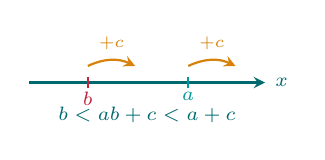
\begin{tikzpicture}[scale=0.75]
      \draw[thick, ->, >=stealth, color=brandNavy] (-0.3,0) -- (3.7,0) node[right, font=\fontsize{7}{7}\selectfont] {$x$};
      \draw[thick, color=brandCrimson] (0.7,-0.1) -- (0.7,0.1) node[below=2pt, font=\fontsize{7.5}{7.5}\selectfont, color=brandCrimson] {$b$};
      \draw[thick, color=koreaTeal] (2.4,-0.1) -- (2.4,0.1) node[below=2pt, font=\fontsize{7.5}{7.5}\selectfont, color=koreaTeal] {$a$};
      \draw[->, >=stealth, color=brandGold, thick] (0.7,0.28) to[bend left=25] node[above, font=\fontsize{6.5}{6.5}\selectfont] {$+c$} (1.5,0.28);
      \draw[->, >=stealth, color=brandGold, thick] (2.4,0.28) to[bend left=25] node[above, font=\fontsize{6.5}{6.5}\selectfont] {$+c$} (3.2,0.28);
      \node[font=\fontsize{7}{7}\selectfont\kml, color=brandNavy] at (1.7,-0.55) {$b < a \implies b+c < a+c$};
    \end{tikzpicture}
  \end{minipage}
\end{khboxorange}

\begin{khboxorange}
  \begin{minipage}[c]{0.68\textwidth}
    \begin{itemize}[leftmargin=12pt, itemsep=1pt, topsep=1pt, parsep=0pt]
      \item[\color{brandNavy}\ding{228}] \textbf{គុណ ឬចែកនឹងចំនួនវិជ្ជមាន ($c > 0$) ៖} បានវិសមភាពថ្មីមានទិសដៅ\textbf{ដូចវិសមភាពដើម} ៖
      \begin{equation*}
        \koreahl{$a > b \quad \text{និង} \quad c > 0 \implies ac > bc \quad \text{និង} \quad a \div c > b \div c$}
      \end{equation*}
      \item[\color{brandCrimson}\ding{228}] \textbf{គុណ ឬចែកនឹងចំនួនអវិជ្ជមាន ($c < 0$) ៖} បានវិសមភាពថ្មីមានទិសដៅ\textbf{ផ្ទុយពីវិសមភាពដើម} ៖
      \begin{equation*}
        \koreahl{$a > b \quad \text{និង} \quad c < 0 \implies ac < bc \quad \text{និង} \quad a \div c < b \div c$}
      \end{equation*}
    \end{itemize}
  \end{minipage}\hfill
  \begin{minipage}[c]{0.30\textwidth}
    \centering
    \begin{tikzpicture}[scale=0.75]
      \draw[thick, ->, >=stealth, color=brandNavy] (-2.2,0) -- (2.2,0) node[right, font=\fontsize{7}{7}\selectfont] {$x$};
      \fill[brandCrimson] (1.2,0) circle (1.8pt) node[below=2pt, font=\fontsize{7.5}{7.5}\selectfont] {$2$};
      \fill[koreaTeal] (-1.2,0) circle (1.8pt) node[below=2pt, font=\fontsize{7.5}{7.5}\selectfont] {$-2$};
      \draw[->, >=stealth, color=brandCrimson, thick] (1.2,0.22) to[bend right=45] node[above, font=\fontsize{6.5}{6.5}\selectfont] {$\times (-1)$} (-1.2,0.22);
      \node[font=\fontsize{7}{7}\selectfont\kml, color=brandCrimson] at (0,-0.55) {គុណនឹង $-1$ ប្ដូរទិសដៅ};
    \end{tikzpicture}
  \end{minipage}
\end{khboxorange}

\vspace{1pt}
\vspace{1pt}
\begin{multicols}{2}
  \noindent
  \exhead{1} \textbf{ចូរបំពេញសញ្ញា ($>, <, \ge, \le$) ក្នុងប្រអប់ ៖}\\
  គេឱ្យ $a > b$ ។ ចូរប្រៀបធៀបគូរនីមួយៗខាងក្រោម ៖\\
  \khlabel{ក} $a + 6$ \ \khboxfill \ $b + 6$ \qquad
  \khlabel{ខ} $a - 4$ \ \khboxfill \ $b - 4$\\
  \khlabel{គ} $a + (-5)$ \ \khboxfill \ $b + (-5)$ \quad
  \khlabel{ឃ} $a - (-8)$ \ \khboxfill \ $b - (-8)$\\
  \khlabel{ង} $a + x$ \ \khboxfill \ $b + x$ \qquad
  \khlabel{ច} $a - y$ \ \khboxfill \ $b - y$
  
  \vspace{4.5pt}
  \exhead{2} \textbf{ចូរបំពេញសញ្ញា ($>, <$) ក្នុងប្រអប់ ៖}\\
  គេឱ្យ $x < y$ ។ ចូរប្រៀបធៀបគូរនីមួយៗខាងក្រោម ៖\\
  \khlabel{ក} $3x$ \ \khboxfill \ $3y$ \qquad\qquad\quad
  \khlabel{ខ} $-3x$ \ \khboxfill \ $-3y$\\
  \khlabel{គ} $\frac{x}{5}$ \ \khboxfill \ $\frac{y}{5}$ \qquad\qquad\quad\ \,
  \khlabel{ឃ} $-\frac{x}{2}$ \ \khboxfill \ $-\frac{y}{2}$\\
  \khlabel{ង} $-7x$ \ \khboxfill \ $-7y$ \qquad\qquad\ 
  \khlabel{ច} $\frac{x}{-10}$ \ \khboxfill \ $\frac{y}{-10}$
  
  \vspace{4.5pt}
  \exhead{3} \textbf{លក្ខណៈបន្សំនៃប្រមាណវិធី ៖}\\
  គេឱ្យ $m \ge n$ ។ ចូរប្រៀបធៀបគូរនីមួយៗ ៖\\
  \khlabel{ក} $2m + 3$ \ \khboxfill \ $2n + 3$ \qquad
  \khlabel{ខ} $-4m + 1$ \ \khboxfill \ $-4n + 1$\\
  \khlabel{គ} $5 - 3m$ \ \khboxfill \ $5 - 3n$ \qquad
  \khlabel{ឃ} $\frac{2m - 1}{3}$ \ \khboxfill \ $\frac{2n - 1}{3}$\\
  \khlabel{ង} $-\frac{m}{4} + 2$ \ \khboxfill \ $-\frac{n}{4} + 2$ \quad
  \khlabel{ច} $10 - 2m$ \ \khboxfill \ $10 - 2n$
  
  \columnbreak
  \noindent
  \exhead{4} \textbf{ស្រាយបញ្ជាក់វិសមភាពពិជគណិត ៖}\\
  \khlabel{ក} ចំពោះគ្រប់ $a, b \in \mathbb{R}$ ស្រាយបញ្ជាក់ថា $a^2 + b^2 \ge 2ab$ ។\\
  \khlabel{ខ} ចំពោះគ្រប់ $x \in \mathbb{R}$ ស្រាយបញ្ជាក់ថា $x^2 + 9 \ge 6x$ ។\\
  \khlabel{គ} ចំពោះគ្រប់ $x \in \mathbb{R}$ ស្រាយបញ្ជាក់ថា $4x^2 + 1 \ge 4x$ ។\\
  \khlabel{ឃ} ចំពោះគ្រប់ $a, b \ge 0$ ស្រាយបញ្ជាក់ថា $(a+b)^2 \ge 4ab$ ។\\
  \khlabel{ង} ចំពោះគ្រប់ $a, b \in \mathbb{R}$ ស្រាយបញ្ជាក់ថា $a^2 + b^2 + 2 \ge 2(a+b)$ ។
  
  \vspace{4.5pt}
  \exhead{5} \textbf{វិសមភាពផលធៀបនៃពីរចំនួន ៖}\\
  \khlabel{ក} គេឱ្យ $a, b \neq 0$ ដែល $ab > 0$ ។ ចូរស្រាយបញ្ជាក់ថា ៖
  \begin{equation*}
    \frac{a}{b} + \frac{b}{a} \ge 2
  \end{equation*}
  \khlabel{ខ} គេឱ្យ $a, b \neq 0$ ដែល $ab < 0$ ។ ចូរស្រាយបញ្ជាក់ថា ៖
  \begin{equation*}
    \frac{a}{b} + \frac{b}{a} \le -2
  \end{equation*}
  \khlabel{គ} គេឱ្យ $x > 0$ ។ ចូរស្រាយបញ្ជាក់ថា $x + \frac{1}{x} \ge 2$ ។\\
  \khlabel{ឃ} គេឱ្យ $x, y > 0$ ។ ចូរស្រាយបញ្ជាក់ថា $\frac{x^2+y^2}{x+y} \ge \frac{x+y}{2}$ ។
  
  \vspace{4.5pt}
  \exhead{6} \textbf{វិសមភាពស្វ័យគុណ និងច្រាស ៖}\\
  គេឱ្យ $a$ និង $b$ ជាពីរចំនួនវិជ្ជមាន ($a > b > 0$) ៖\\
  \khlabel{ក} ស្រាយបញ្ជាក់ថា $a^2 > b^2$ ។\\
  \khlabel{ខ} ស្រាយបញ្ជាក់ថា $a^3 > b^3$ ។\\
  \khlabel{គ} ស្រាយបញ្ជាក់ថា $\frac{1}{a} < \frac{1}{b}$ ។\\
  \khlabel{ឃ} ស្រាយបញ្ជាក់ថា $\frac{a}{a+1} > \frac{b}{b+1}$ ។
\end{multicols}

\newpage

% =========================================================================
% PAGE 2: ផ្នែកទី ២ ៖ វិសមីការដឺក្រេទី១ មានមួយអញ្ញាត (Two-column Korean Style)
% =========================================================================
\khsection{២}{វិសមីការដឺក្រេទី១ មានមួយអញ្ញាត (Linear Inequalities in One Variable)}

\begin{khcard}
  \noindent
  \textbf{\ding{228} សញ្ញាណវិសមីការ និងចម្លើយ ៖} រក $x$ ដែល $x + 4 = 7$ (សមីការមានចម្លើយ $x = 3$) ។ រក $x$ ដែល $x + 4 < 7$ (វិសមីការដឺក្រេទី១ មានមួយអញ្ញាត $x$) ៖
  \vspace{1pt}
  \begin{center}
  \fontsize{7}{7}\selectfont
  \begin{tabular}{|l|l|l||l|l|l|}
    \hline
    \rowcolor{brandNavy!10}
    \textbf{តម្លៃ $x$} & \textbf{ការជំនួសចូល $x+4 < 7$} & \textbf{ការសន្និដ្ឋាន} & \textbf{តម្លៃ $x$} & \textbf{ការជំនួសចូល $x+4 < 7$} & \textbf{ការសន្និដ្ឋាន} \\ \hline
    $x = 4$ & $4 + 4 = 8 > 7$ (មិនផ្ទៀងផ្ទាត់) & $x = 4$ \textbf{មិនមែនជាចម្លើយ} & $x = 1$ & $1 + 4 = 5 < 7$ (ផ្ទៀងផ្ទាត់) & $x = 1$ \textbf{ជាចម្លើយ} \\ \hline
    $x = 3$ & $3 + 4 = 7 = 7$ (មិនផ្ទៀងផ្ទាត់) & $x = 3$ \textbf{មិនមែនជាចម្លើយ} & $x = 0$ & $0 + 4 = 4 < 7$ (ផ្ទៀងផ្ទាត់) & $x = 0$ \textbf{ជាចម្លើយ} \\ \hline
    $x = 2$ & $2 + 4 = 6 < 7$ (ផ្ទៀងផ្ទាត់) & $x = 2$ \textbf{ជាចម្លើយ} & $x = -1$ & $-1 + 4 = 3 < 7$ (ផ្ទៀងផ្ទាត់) & $x = -1$ \textbf{ជាចម្លើយ} \\ \hline
  \end{tabular}
  \end{center}
  \vspace{-1pt}
  \noindent
  $\implies$ មានតម្លៃ $x$ រាប់មិនអស់ដែលផ្ទៀងផ្ទាត់វិសមីការ ។ សំណុំចម្លើយបកស្រាយដោយវិសមភាពគឺ \koreahl{$x < 3$} ។
\end{khcard}

\begin{khboxorange}
  \begin{minipage}[c]{0.65\textwidth}
    \begin{itemize}[leftmargin=12pt, itemsep=1.2pt, topsep=1pt, parsep=0pt]
      \item[\color{brandNavy}\ding{228}] \textbf{ទម្រង់ទូទៅ ៖} $ax + b > 0$, \ $ax + b < 0$, \ $ax + b \ge 0$, \ $ax + b \le 0$ \ ($a \neq 0$)
      \item[\color{brandCrimson}\ding{228}] \textbf{វិធានដោះស្រាយ ៖} ផ្ទេរតួអញ្ញាត $x$ ទៅអង្គខាងឆ្វេង និងចំនួនថេរទៅអង្គខាងស្ដាំ រួចចែកនឹង $a$ (បើ $a < 0$ ត្រូវ\textbf{ត្រឡប់ទិសដៅវិសមីការ}) ។
      \item[\color{brandGold}\ding{228}] \textbf{ក្រាបលើបន្ទាត់ចំនួន ៖} ប្រើ `)' ឬ `(' បញ្ជាក់ថា\textbf{មិនយកជាចម្លើយ} ($<, >$), ប្រើ `]' ឬ `[' បញ្ជាក់ថា\textbf{យកជាចម្លើយ} ($\le, \ge$) ។
    \end{itemize}
  \end{minipage}\hfill
  \begin{minipage}[c]{0.33\textwidth}
    \centering
    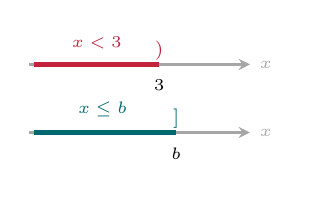
\begin{tikzpicture}[scale=0.72]
      \draw[thick, ->, >=stealth, color=gray!70] (-0.3,1.5) -- (3.6,1.5) node[right, font=\fontsize{6}{6}\selectfont] {$x$};
      \draw[ultra thick, color=brandCrimson] (-0.2,1.5) -- (2.0,1.5);
      \node[above, font=\fontsize{7.5}{7.5}\selectfont, color=brandCrimson] at (2.0,1.4) {$)$};
      \node[below=1pt, font=\fontsize{6.5}{6.5}\selectfont] at (2.0,1.45) {$3$};
      \node[above=1pt, font=\fontsize{6.5}{6.5}\selectfont\kml, color=brandCrimson] at (0.9,1.55) {$x < 3$};
      
      \draw[thick, ->, >=stealth, color=gray!70] (-0.3,0.3) -- (3.6,0.3) node[right, font=\fontsize{6}{6}\selectfont] {$x$};
      \draw[ultra thick, color=brandNavy] (-0.2,0.3) -- (2.3,0.3);
      \node[above, font=\fontsize{7.5}{7.5}\selectfont, color=brandNavy] at (2.3,0.2) {$]$};
      \node[below=1pt, font=\fontsize{6.5}{6.5}\selectfont] at (2.3,0.25) {$b$};
      \node[above=1pt, font=\fontsize{6.5}{6.5}\selectfont\kml, color=brandNavy] at (1.0,0.35) {$x \le b$};
    \end{tikzpicture}
  \end{minipage}
\end{khboxorange}

\vspace{1pt}
\begin{multicols}{2}
  \noindent
  \exhead{1} \textbf{ប្រភេទទី ១ ៖ វិសមីការសាមញ្ញ (បូក ដក គុណ ចែក) ៖}\\
  \textit{\fontsize{7.5}{7.5}\selectfont\color{brandNavy}ចូរដោះស្រាយវិសមីការ និងបកស្រាយចម្លើយតាមក្រាបបន្ទាត់ចំនួន ៖}\\
  \khlabel{ក} $x - 2 < 5$\\
  \khlabel{ខ} $x + 5 \ge 3$\\
  \khlabel{គ} $3 - x < 7 - 2x$\\
  \khlabel{ឃ} $5x \ge 10$\\
  \khlabel{ង} $-3x + 1 < 7$\\
  \khlabel{ច} $-6x < 12$\\
  \khlabel{ឆ} $-5x > -20$\\
  \khlabel{ជ} $2x \le -\frac{1}{3}$\\
  \khlabel{ឈ} $4x - 7 \le 5$\\
  \khlabel{ញ} $-2x - 5 \ge 3$\\
  \khlabel{ដ} $-5x + 4 \le -11$\\
  \khlabel{ឋ} $3x - 5 < x + 7$\\
  \khlabel{ឌ} $7x + 12 \ge 3x - 8$\\
  \khlabel{ឍ} $-4x + 15 < -2x + 7$

  \vspace{4.5pt}
  \exhead{2} \textbf{ប្រភេទទី ២ ៖ វិសមីការមានគុណកត្តា (វង់ក្រចក) ៖}\\
  \textit{\fontsize{7.5}{7.5}\selectfont\color{brandNavy}ចូរដោះស្រាយវិសមីការ និងបកស្រាយចម្លើយតាមក្រាបបន្ទាត់ចំនួន ៖}\\
  \khlabel{ក} $2(x - 1) < 8$\\
  \khlabel{ខ} $2(x + 3) > 5x + 5$\\
  \khlabel{គ} $-2x - 1 \ge 2\left(x + \frac{1}{2}\right)$\\
  \khlabel{ឃ} $3(2x - 1) - 4(x + 2) \le 5$\\
  \khlabel{ង} $4(x - 2) \ge 3(2x + 1) - 5$\\
  \khlabel{ច} $5(2x - 3) - 2(x - 1) > 3(x + 4)$\\
  \khlabel{ឆ} $3(x - 4) + 2(3x + 1) \ge 4(2x - 1)$\\
  \khlabel{ជ} $2(3 - 2x) - 5(1 - x) < 3(x + 2)$\\
  \khlabel{ឈ} $0.5(x - 2) - 0.2(3x + 1) < 1.4$\\
  \khlabel{ញ} $0.37x + 0.17 > 3.5$\\
  \khlabel{ដ} $1.2(x + 5) - 0.8(2x - 1) \ge 3.4$\\
  \khlabel{ឋ} $(x + 2)^2 - x^2 \le 4x + 16$

  \columnbreak
  \noindent
  \exhead{3} \textbf{ប្រភេទទី ៣ ៖ វិសមីការមានភាគបែង (តម្រូវភាគបែង) ៖}\\
  \textit{\fontsize{7.5}{7.5}\selectfont\color{brandNavy}ចូរដោះស្រាយវិសមីការ និងបកស្រាយចម្លើយតាមក្រាបបន្ទាត់ចំនួន ៖}\\
  \khlabel{ក} $\frac{x}{7} > \frac{1}{4}$\\
  \khlabel{ខ} $\frac{1}{2}x > 4$\\
  \khlabel{គ} $-\frac{2}{3}x \le 6$\\
  \khlabel{ឃ} $-3x \ge \frac{9}{2}$\\
  \khlabel{ង} $\frac{2x - 1}{3} \ge 1$\\
  \khlabel{ច} $\frac{3 - x}{4} < 2$\\
  \khlabel{ឆ} $\frac{x}{4} + 2 > 7$\\
  \khlabel{ជ} $\frac{2}{3}x + 3 > \frac{5}{3}x - 27$\\
  \khlabel{ឈ} $\frac{x+1}{2} < \frac{2x - 3}{4}$\\
  \khlabel{ញ} $x - \frac{1 + 2x}{4} \ge \frac{1 - 3x}{3}$\\
  \khlabel{ដ} $\frac{x+1}{5} - \frac{1}{2} \le \frac{3 + 2x}{2}$\\
  \khlabel{ឋ} $\frac{3x - 1}{2} - \frac{x + 2}{3} > \frac{x}{6} + 1$\\
  \khlabel{ឌ} $\frac{2x - 5}{3} - \frac{x - 2}{4} \le \frac{3x + 1}{6}$\\
  \khlabel{ឍ} $\frac{x - 1}{2} - \frac{2x + 3}{3} \ge \frac{x}{6} - 2$\\
  \khlabel{ណ} $\frac{3(x - 2)}{4} - \frac{2(x + 1)}{3} < \frac{x - 5}{12}$\\
  \khlabel{ត} $\frac{5x - 2}{6} - \frac{2x + 1}{4} > \frac{x - 3}{3} - 1$\\
  \khlabel{ថ} $\frac{4x + 1}{5} - \frac{3(x - 1)}{2} \le \frac{2x - 7}{10}$\\
  \khlabel{ទ} $\frac{x+3}{2} - \frac{x-1}{3} \ge \frac{2x+5}{6}$\\
  \khlabel{ធ} $\frac{2(x-3)}{5} + \frac{3(x+1)}{2} > \frac{7x-1}{10} + 2$\\
  \khlabel{ន} $\frac{x-4}{3} - \frac{2x-1}{5} < \frac{3x+2}{15} - 1$
\end{multicols}

\newpage

% =========================================================================
% PAGE 3: ផ្នែកទី ៣ & ផ្នែកទី ៤ (Two-column Korean Style)
% =========================================================================
\khsection{៣}{ប្រព័ន្ធវិសមីការដឺក្រេទី១ មានមួយអញ្ញាត (Systems of Linear Inequalities)}

\begin{khboxorange}
  \begin{minipage}[c]{0.68\textwidth}
    \begin{itemize}[leftmargin=12pt, itemsep=1.5pt, topsep=1pt, parsep=0pt]
      \item[\color{brandNavy}\ding{228}] \textbf{ដំណោះស្រាយនៃប្រព័ន្ធវិសមីការ ៖} គឺជាសំណុំតម្លៃ $x$ ដែលផ្ទៀងផ្ទាត់គ្រប់វិសមីការនៃប្រព័ន្ធព្រមគ្នា (\textbf{ប្រសព្វនៃសំណុំចម្លើយ} $S = S_1 \cap S_2$) ។
      \item[\color{brandCrimson}\ding{228}] \textbf{វិធីសាស្ត្រ ៖} ដោះស្រាយវិសមីការនីមួយៗ រួចគូសបកស្រាយលើបន្ទាត់ចំនួនដើម្បីកំណត់រកចន្លោះរួម ។
    \end{itemize}
  \end{minipage}\hfill
  \begin{minipage}[c]{0.30\textwidth}
    \centering
    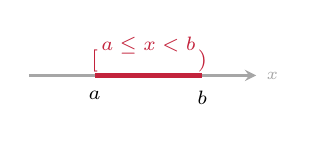
\begin{tikzpicture}[scale=0.76]
      \draw[thick, ->, >=stealth, color=gray!70] (-0.3,0) -- (3.5,0) node[right, font=\fontsize{6.5}{6.5}\selectfont] {$x$};
      \draw[ultra thick, color=brandCrimson] (0.8,0) -- (2.6,0);
      \node[above, font=\fontsize{8}{8}\selectfont, color=brandCrimson] at (0.8,-0.1) {$[$};
      \node[below=1pt, font=\fontsize{7.5}{7.5}\selectfont] at (0.8,-0.05) {$a$};
      \node[above, font=\fontsize{8}{8}\selectfont, color=brandCrimson] at (2.6,-0.1) {$)$};
      \node[below=1pt, font=\fontsize{7.5}{7.5}\selectfont] at (2.6,-0.05) {$b$};
      \node[above=1pt, font=\fontsize{7.5}{7.5}\selectfont\kml, color=brandCrimson] at (1.7,0.15) {$a \le x < b$};
    \end{tikzpicture}
  \end{minipage}
\end{khboxorange}

\khsection{៤}{ចំណោទវិសមីការ (Inequality Word Problems)}

\begin{khcard}
  \noindent
  \textbf{\ding{228} វិធីដោះស្រាយចំណោទវិសមីការ ៖} \textbf{(១)} កំណត់អញ្ញាត $x$ និងលក្ខខណ្ឌ $\to$ \textbf{(២)} បង្កើតវិសមីការតាមប្រធាន $\to$ \textbf{(៣)} ដោះស្រាយវិសមីការ $\to$ \textbf{(៤)} ផ្ទៀងផ្ទាត់លក្ខខណ្ឌ និងសន្និដ្ឋានចម្លើយ ។
\end{khcard}

\vspace{1pt}
\begin{multicols}{2}
  \noindent
  \exhead{1} \textbf{ដោះស្រាយប្រព័ន្ធវិសមីការ ៖}\\
  \khlabel{ក} $\begin{cases} 2x + 5 \ge 5x - 4 \\ x - 7 \ge 2x - 3 \end{cases}$\\
  \khlabel{ខ} $\begin{cases} 3x + 2 > x - 4 \\ 2x - 1 \le 5x + 8 \end{cases}$

  \vspace{3pt}
  \exhead{2} \textbf{ប្រព័ន្ធវិសមីការកម្រិតគ្រឹះ ៖}\\
  \khlabel{ក} $\begin{cases} 2x - 3 \le 9 \\ 2x - 3 \ge -5 \end{cases}$\\
  \khlabel{ខ} $\begin{cases} 3x - 4 \le 8 \\ 3x - 4 > -7 \end{cases}$\\
  \khlabel{គ} $\begin{cases} 2x + 5 > 5x - 4 \\ x - 7 < 2x - 3 \end{cases}$\\
  \khlabel{ឃ} $\begin{cases} 4x + 1 \ge 9 \\ 3x - 2 < 13 \end{cases}$

  \vspace{3pt}
  \exhead{3} \textbf{ប្រព័ន្ធវិសមីការកម្រិតមធ្យម ៖}\\
  \khlabel{ក} $\begin{cases} 2x - 3 > 5x - 1 \\ x + 4 \ge 3x - 2 \end{cases}$\\
  \khlabel{ខ} $\begin{cases} \frac{3x}{4} - \frac{2}{3} \le \frac{4x - 3}{2} \\[2pt] 2x - 1 > \frac{3x - 4}{4} \end{cases}$\\
  \khlabel{គ} $\begin{cases} 2x + 1 < 0 \\ -\frac{x}{2} + 2 < 0 \end{cases}$\\
  \khlabel{ឃ} $\begin{cases} \frac{x-1}{2} \ge \frac{x+1}{3} \\ 2(x+3) > 3x - 1 \end{cases}$

  \vspace{3pt}
  \exhead{4} \textbf{ដោះស្រាយប្រព័ន្ធវិសមីការ ៖}\\
  \khlabel{ក} $\begin{cases} 2x - 7 \le 6x + 5 \\ 4x - 11 \le 4 + x \end{cases}$\\
  \khlabel{ខ} $\begin{cases} \frac{3x}{4} - \frac{2}{3} \le \frac{4x - 3}{12} \\[2pt] 2x - 1 > \frac{3x - 4}{2} \end{cases}$\\
  \khlabel{គ} $\begin{cases} 3(x-2) \le 2(x+1) \\ \frac{2x+1}{5} < \frac{x-2}{2} \end{cases}$

  \columnbreak
  \noindent
  \exhead{5} \textbf{វិមាត្រនៃចតុកោណកែង ៖}\\
  ចតុកោណកែងមួយមានវិមាត្រទទឹង $x$ និងបណ្ដោយ $x+2$ (គិតជា $\text{m}$) ដូចរូប ($x > 0$) ៖
  \begin{center}
  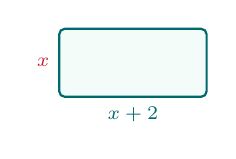
\begin{tikzpicture}[scale=0.72]
    \draw[thick, fill=brandTealBg, draw=brandNavy, rounded corners=2pt] (0,0) rectangle (2.6,1.2);
    \node[left, font=\fontsize{7.5}{7.5}\selectfont, color=brandCrimson] at (0,0.6) {$x$};
    \node[below, font=\fontsize{7.5}{7.5}\selectfont, color=brandNavy] at (1.3,0) {$x + 2$};
  \end{tikzpicture}
  \end{center}
  \khlabel{ក} រកតម្លៃ $x$ ដើម្បីឱ្យបរិមាត្រធំជាង $32\,\text{m}$ ។\\
  \khlabel{ខ} រកតម្លៃ $x$ ដើម្បីឱ្យបរិមាត្រតូចជាង $32\,\text{m}$ ។\\
  \khlabel{គ} រកតម្លៃ $x$ ដើម្បីឱ្យផ្ទៃក្រឡាធំជាង ឬស្មើ $15\,\text{m}^2$ (បើ $x$ ជាចំនួនគត់) ។

  \vspace{4pt}
  \exhead{6} \textbf{ចំណោទអាយុ ៖}\\
  \khlabel{ក} ពូសុខមានអាយុច្រើនជាងកូន $32$ ឆ្នាំ និងតិចជាងឪពុក $33$ ឆ្នាំ ។ ផលបូកអាយុអ្នកទាំងបី $< 103$ ឆ្នាំ ។ ចូររកអាយុពូសុខ បើអាយុគាត់ជាចំនួនគត់ ។\\
  \khlabel{ខ} ម្ដាយមានអាយុច្រើនជាងកូន $25$ ឆ្នាំ ។ ចូររកអាយុកូន បើផលបូកអាយុអ្នកទាំងពីរតិចជាង $55$ ឆ្នាំ ហើយអាយុកូនធំជាង $12$ ឆ្នាំ (អាយុជាចំនួនគត់) ។

  \vspace{4pt}
  \exhead{7} \textbf{ចំណោទអនុវត្ត ៖}\\
  \khlabel{ក} គេឱ្យចតុកោណកែងមួយមានទទឹង $5\,\text{m}$ និងបណ្ដោយ $x\,\text{m}$ ។ តើ $x$ ត្រូវយកតម្លៃណាខ្លះ ដើម្បីឱ្យបរិមាត្រធំជាង $18\,\text{m}$ និងផ្ទៃក្រឡាតូចជាង $50\,\text{m}^2$ ?\\
  \khlabel{ខ} ផលបូកនៃបីចំនួនគត់តគ្នាតូចជាង $1918$ តែធំជាង $1914$ ។ ចូររកចំនួនទាំងបីនោះ ។\\
  \khlabel{គ} ផលបូកនៃពីរចំនួនគត់គូតគ្នាតូចជាង $50$ តែធំជាង $42$ ។ ចូររកចំនួនទាំងពីរនោះ ។
\end{multicols}

\newpage

% =========================================================================
% PAGE 4: កម្រងលំហាត់អនុវត្តន៍ពេញលេញ ១៣ លំហាត់ តាមសៀវភៅពុម្ពក្រសួង
% =========================================================================
\noindent
\begin{tikzpicture}
  \fill[rounded corners=5pt, brandNavy] (0,0) rectangle (19.3, 0.58);
  \node[white, font=\fontsize{10.5}{10.5}\selectfont\kml\bfseries] at (9.65, 0.29) {\ding{72}\ \ កម្រងលំហាត់អនុវត្តន៍ និងត្រៀមប្រឡងប្រចាំមេរៀន (សៀវភៅពុម្ពក្រសួង) \ \ \ding{72}};
\end{tikzpicture}

\vspace{2pt}
\begin{multicols}{2}
  \noindent
  \exhead{1} \badgebasic\\
  គេដាំកូនឈើចំនួន $40$ ដើមព័ទ្ធជុំវិញចំការមួយរាងចតុកោណកែង ។ តើចំការនោះអាចមានផ្ទៃក្រឡាធំបំផុតប៉ុន្មាន $\text{m}^2$ បើគេដឹងថា គេដាំកូនឈើឃ្លាតពីគ្នា $2\,\text{m}$ ?
  
  \vspace{3.5pt}
  \exhead{2} \badgebasic\\
  ចូរបង្ហាញថាជ្រុងនីមួយៗនៃត្រីកោណ មានប្រវែងខ្លីជាងកន្លះបរិមាត្រនៃត្រីកោណនោះ ($a < p, \ b < p, \ c < p$ ដែល $p = \frac{a+b+c}{2}$) ។
  
  \vspace{3.5pt}
  \exhead{3} \badgebasic\\
  ពាក់កណ្ដាលនៃមួយចំនួនថែមនឹង $5$ ធំជាង ឬស្មើនឹង $-3$ ។ ចូររកចំនួននោះ ។
  
  \vspace{3.5pt}
  \exhead{4} \badgestandard\\
  បច្ចុប្បន្ននេះឪពុកមានអាយុ $32$ ឆ្នាំ ហើយកូនគាត់មានអាយុ $12$ ឆ្នាំ ។ តើនៅក្នុងចន្លោះប៉ុន្មានឆ្នាំទៅមុខទៀត ទើបអាយុឪពុកតិចជាងបីដង ប៉ុន្តែច្រើនជាងពីរដងនៃអាយុកូន ?
  
  \vspace{3.5pt}
  \exhead{5} \badgeadvanced\\
  សុខមានក្រដាសប្រាក់ពីរដុំ ៖ ដុំទី ១ មានក្រដាស $500\,\text{៛}$ ចំនួន $20$ សន្លឹក និងដុំទី ២ មានក្រដាស $1000\,\text{៛}$ ចំនួន $30$ សន្លឹក ។ ថ្ងៃមួយសុខដកយក $25$ សន្លឹកពីដុំទាំងពីរ ។ បើសុខចង់បានប្រាក់សរុបយ៉ាងតិច $17\,500\,\text{៛}$ និងយ៉ាងច្រើន $20\,000\,\text{៛}$ តើសុខអាចមានក្រដាសប្រាក់ $500\,\text{៛}$ ប៉ុន្មានសន្លឹក ?
  
  \vspace{3.5pt}
  \exhead{6} \badgestandard\\
  ក្នុងការប្រឡងលើ $8$ មុខវិជ្ជា (មួយមុខ $100$ ពិន្ទុ) និទ្ទេស $A$ ទាល់តែមធ្យមភាគ $\ge 90$ និងនិទ្ទេស $B$ មធ្យមភាគ $\ge 80$ ។ វិសាលប្រឡងបាន $7$ មុខទទួលបានពិន្ទុ $84, 93, 78, 87, 89, 70, 81$ ៖\\
  \khlabel{ក} តើវិសាលអាចទទួលបាននិទ្ទេស $A$ ឬទេ ?\\
  \khlabel{ខ} កំណត់ពិន្ទុមុខចុងក្រោយដើម្បីឱ្យវិសាលបាននិទ្ទេស $B$ ។
  
  \vspace{3.5pt}
  \exhead{7} \badgestandard\\
  សួនមួយមានរាងចតុកោណកែង ។ បណ្ដោយមានរង្វាស់លើស $3$ ដងនៃទទឹងប្រវែង $15\,\text{m}$ ។ ដោយដឹងថាបរិមាត្រនៃសួនវែងបំផុតស្មើនឹង $94\,\text{m}$ ចូររកបរិមាត្រអតិបរមានៃសួននោះ បើរង្វាស់ជ្រុងជាចំនួនគត់ ។
  
  \columnbreak
  \noindent
  \exhead{8} \badgestandard\\
  សំបុត្រដែលត្រូវលក់ឱ្យភ្ញៀវមានពីរប្រភេទ A និង B ដែលប្រភេទ A មានចំនួនលើសប្រភេទ B ចំនួន $5$ សន្លឹក ។ បើគេលក់សំបុត្រយ៉ាងច្រើនបាន $37$ សន្លឹក ចូររកចំនួនសំបុត្រនៃប្រភេទនីមួយៗដែលអាចលក់បានច្រើនបំផុត ។
  
  \vspace{3.5pt}
  \exhead{9} \badgebasic\\
  ផលបូកនៃពីរចំនួនគត់សេសតគ្នាតូចបំផុត $72$ ។ ចូរកំណត់ចំនួនគត់សេសទាំងពីរដែលមានតម្លៃធំជាងគេ ។
  
  \vspace{3.5pt}
  \exhead{10} \badgeadvanced\\
  លក្ខខណ្ឌជួលរថយន្ត ៖ ឈ្នួលក្នុង $1$ ថ្ងៃថ្លៃ $80\,000\,\text{៛}$ ព្រមទាំងប្រាក់បន្ថែម $400\,\text{៛}$ ក្នុងចម្ងាយផ្លូវ $1\,\text{km}$ ។ អ្នកជួលបានកក់ប្រាក់ $400\,000\,\text{៛}$ សម្រាប់ $1$ ថ្ងៃ ។ តើអ្នកជួលត្រូវបើកបរចម្ងាយផ្លូវយ៉ាងច្រើនប៉ុន្មាន $\text{km}$ ដើម្បីកុំឱ្យឈ្នួលជួលលើសពីប្រាក់កក់ ?
  
  \vspace{3.5pt}
  \exhead{11} \badgeadvanced\\
  គេឱ្យត្រីកោណ $ABC$ ដែលមានជ្រុង $AB = 12\,\text{cm}$ និង $AC = 3\,\text{cm}$ ។ តើជ្រុង $BC$ អាចមានប្រវែងប៉ុន្មាន បើដឹងថាប្រវែង $BC$ ជាចំនួនគត់ពហុគុណនៃ $3$ ?
  
  \vspace{3.5pt}
  \exhead{12} \badgebasic\\
  ចូររកចំនួនគត់ដែលពីរដងនៃតម្លៃរបស់វាយ៉ាងតិចស្មើនឹង $8$ ($2x \ge 8$) ។
  
  \vspace{3.5pt}
  \exhead{13} \badgestandard\\
  បូណាមានក្រដាសរាងចតុកោណកែងទទឹង $3\,\text{cm}$ និងផ្ទៃក្រឡានៅចន្លោះពី $15\,\text{cm}^2$ ទៅ $24\,\text{cm}^2$ ។ តើបូណាត្រូវជ្រើសរើសបណ្ដោយប្រវែងប៉ុន្មានខ្លះ បើបណ្ដោយជាចំនួនគត់ ?
\end{multicols}

\vfill
\begin{center}
  \begin{tikzpicture}
    \node[draw=brandTeal, fill=brandTealBg, rounded corners=6pt, inner sep=4.5pt, text=brandNavy, font=\fontsize{8}{8}\selectfont\kml] {
      \ding{72}\ \textbf{ស្វ័យសិក្សា និងការអនុវត្តជាប្រចាំ នាំមកនូវឧត្តមភាពក្នុងការដោះស្រាយវិសមីការគណិតវិទ្យា} \ \ding{72}
    };
  \end{tikzpicture}
\end{center}

\end{document}
